\documentclass{article}\usepackage[]{graphicx}\usepackage[]{color}
%% maxwidth is the original width if it is less than linewidth
%% otherwise use linewidth (to make sure the graphics do not exceed the margin)
\makeatletter
\def\maxwidth{ %
  \ifdim\Gin@nat@width>\linewidth
    \linewidth
  \else
    \Gin@nat@width
  \fi
}
\makeatother

\definecolor{fgcolor}{rgb}{0.345, 0.345, 0.345}
\newcommand{\hlnum}[1]{\textcolor[rgb]{0.686,0.059,0.569}{#1}}%
\newcommand{\hlstr}[1]{\textcolor[rgb]{0.192,0.494,0.8}{#1}}%
\newcommand{\hlcom}[1]{\textcolor[rgb]{0.678,0.584,0.686}{\textit{#1}}}%
\newcommand{\hlopt}[1]{\textcolor[rgb]{0,0,0}{#1}}%
\newcommand{\hlstd}[1]{\textcolor[rgb]{0.345,0.345,0.345}{#1}}%
\newcommand{\hlkwa}[1]{\textcolor[rgb]{0.161,0.373,0.58}{\textbf{#1}}}%
\newcommand{\hlkwb}[1]{\textcolor[rgb]{0.69,0.353,0.396}{#1}}%
\newcommand{\hlkwc}[1]{\textcolor[rgb]{0.333,0.667,0.333}{#1}}%
\newcommand{\hlkwd}[1]{\textcolor[rgb]{0.737,0.353,0.396}{\textbf{#1}}}%
\let\hlipl\hlkwb

\usepackage{framed}
\makeatletter
\newenvironment{kframe}{%
 \def\at@end@of@kframe{}%
 \ifinner\ifhmode%
  \def\at@end@of@kframe{\end{minipage}}%
  \begin{minipage}{\columnwidth}%
 \fi\fi%
 \def\FrameCommand##1{\hskip\@totalleftmargin \hskip-\fboxsep
 \colorbox{shadecolor}{##1}\hskip-\fboxsep
     % There is no \\@totalrightmargin, so:
     \hskip-\linewidth \hskip-\@totalleftmargin \hskip\columnwidth}%
 \MakeFramed {\advance\hsize-\width
   \@totalleftmargin\z@ \linewidth\hsize
   \@setminipage}}%
 {\par\unskip\endMakeFramed%
 \at@end@of@kframe}
\makeatother

\definecolor{shadecolor}{rgb}{.97, .97, .97}
\definecolor{messagecolor}{rgb}{0, 0, 0}
\definecolor{warningcolor}{rgb}{1, 0, 1}
\definecolor{errorcolor}{rgb}{1, 0, 0}
\newenvironment{knitrout}{}{} % an empty environment to be redefined in TeX

\usepackage{alltt}

\usepackage{fancyhdr} % Required for custom headers
\usepackage{lastpage} % Required to determine the last page for the footer
\usepackage{extramarks} % Required for headers and footers
\usepackage{graphicx} % Required to insert images
\usepackage{hyperref}
\usepackage{amsmath} %for binomial pdf
\usepackage{parskip} % so that there's space bw paragraphs
\usepackage{float}
\usepackage{amsfonts}
\usepackage{verbatim}
\graphicspath{"~/almhub_0823/exp_design/project"}



% Margins
\topmargin=-0.45in
\evensidemargin=0in
\oddsidemargin=0in
\textwidth=6.5in
\textheight=9.0in
\headsep=0.25in 

\linespread{1.1} % Line spacing

% Set up the header and footer
\pagestyle{fancy}
\lhead{STAT 541: Experimental Design} % Top left header
\chead{Project Proposal} % Top center header
\rhead{Andrea Mack} % Top right header
\lfoot{03/08/2017} % Bottom left footer
\cfoot{} % Bottom center footer
\rfoot{Page\ \thepage\ of\ \pageref{LastPage}} % Bottom right footer
\renewcommand\headrulewidth{0.4pt} % Size of the header rule
\renewcommand\footrulewidth{0.4pt} % Size of the footer rule

\setlength\parindent{0pt} % Removes all indentation from paragraphs
\setlength\parskip{0.5cm}
\restylefloat{table}

%----------------------------------------------------------------------------------------
%	DOCUMENT STRUCTURE COMMANDS
%	Skip this unless you know what you're doing
%----------------------------------------------------------------------------------------

% Header and footer for when a page split occurs within a problem environment
\newcommand{\enterProblemHeader}[1]{
\nobreak\extramarks{#1}{#1 continued on next page\ldots}\nobreak
\nobreak\extramarks{#1 (continued)}{#1 continued on next page\ldots}\nobreak
}

% Header and footer for when a page split occurs between problem environments
\newcommand{\exitProblemHeader}[1]{
\nobreak\extramarks{#1 (continued)}{#1 continued on next page\ldots}\nobreak
\nobreak\extramarks{#1}{}\nobreak
}


%----------------------------------------------------------------------------------------%
\IfFileExists{upquote.sty}{\usepackage{upquote}}{}
\begin{document}



\section{Background}

Weaker chicken egg shells are undesirable in appearance for consumers and in handling for distribution and sale companies. Of interest is to compare shell strength between three different brands of eggs. Eggs will be submerged in two concentrations of vinegar solutions. Vinegar contains acetic acid which is known for its properties that break down calcium found in egg shells. The USDA grades chicken eggs (B,A,AA) on both intrinsic and extrinsic factors. Both A and AA grade eggs have the same shell quality requirements. Color also is not a grading factor.

In a $2X3$ crossed factorial design, I will examine the effect of solution on shell strength for different egg brands. Each solution by brand combination will contain 3 replicates. For the analysis, I will treat the two factors as one with six levels.

\subsection{Factors}

1) Brand -- Store brand Grade A (white) , Egglands' best Grade AA (white), Simple truth cage free large brown Grade AA
Note: Brand may vary depending on sale at the time of purchase.

2) Solution -- 100\% vinegar, 50\% water + 50\% vinegar

Note: It is assumed an egg submerged in a 100\% water solution will not change and I will not test this.

\subsection{Response Variables}

The response variable is a proxy for shell strength. Eggs will be dropped horizontally beginning at 1/2 an inch and increasing by 1/2 inch increments. The response variable is height in inches in which the egg breaks.


\begin{center}
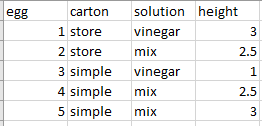
\includegraphics{spreadex}
\end{center}


\section{Protocol}

\subsection{Materials}

The one dozen eggs from each of the three brands of eggs will be bought from a local store. The cheapest white distilled vinegar will also be bought from the same store. Enough of the solutions will be purchased to conduct the experiment. Eggs will be stored in a refrigerator until the experiment begins. 

Solo cups will be used, one for each egg. The amount of solution for each submerged egg will be the same for all eggs. The amount used will be recorded. Plastic wrap will be used to cover the cups to minimize smell and evaporation.

\subsection{Randomization}

Six eggs will randomly be chosen from each carton. The randomization will occur by numbering each egg in 12 value increments from 1 to 36 by carton. A random number generator will sample from 1 to 12 without replacement 6 times, from 13 to 24 without replacement 6 times, and from 25 to 36 without replacement 6 times. Each egg chosen will randomly be assigned a cup. Cups will be filled with solution and labelled so that solution contents are identifiable. Cups will be labelled for solution as follows:

1 = 50\% water + 50\% vinegar

2 = 100\% vinegar

Cups will be labelled 1 to 18. A vector containing six 1's, six 2's, and six 3's will be created, call it {\it solution}. I will sample randomly without replacement from {\it solution} and in the order of occurrence, assign each cup the randomly generated solution and label each cup with either a 1 or 2 label solution as above. Each cup now has a number 1 to 18 and either a 1 or 2 on it.

Recall each egg has a number 1 to 18. Eggs within cartons will be assigned solutions in increasing order. A vector {\it solution2} will be created that contains three 1's and three 2's. Cups will be lined up in increasing order. Assignment will occur by order of types of eggs listed above. Eggs will be assigned to solution (cup) as follows:

For the lowest numbered egg from the store brand carton, a random number from {\it solution2} will be generated. The first cup when lined in increasing order with the corresponding randomly chosen number from {\it solution2} will be assigned for that egg. Numbers will not be replaced and  this method will occur through the largest egg number in the Simple truth egg carton.

\subsection{Experiment}

Each egg will be placed in its respective cup at the same time on the same day. Cups (eggs) will be stored in Andrea's apartment. Cups will be placed in a 6*3 rectangle in no particular order on her kitchen counter away from her stove and water. Environmental temperatures will change throughout the experiment, but will be the same for all cups. Cups will not be placed in direct sunlight and will remain untouched throughout the experiment.

\subsection{Response Data Collection}
Eggs will be submerged in solution for 30 hours. Eggs will then be removed from solution, dried, and any loose shell will be wiped away gently. Eggs will then be dropped in 1/2 inch increments as described above. Height at which the egg explodes will be the response. Once eggs have exploded, the cups will be cleaned and removed from the experimental area.

\section{Proposed Analyses}

\subsection{Plots}

\begin{itemize}

\item Plot response on y axis, solution type on x axis, color points by egg type.

\item Interaction plot
\end{itemize}

\subsection{Modelling}

The model used includes one factor with six levels:

\begin{center}
$y_{ij} = \mu + \beta_{i} + \epsilon_{ij}$
\end{center}

Parameterization will be based on SAS's constraints.

i = 1,...,6

j = 1,2,3

$y_{ij}$ = height at explosion 

$\mu$ = mean explosion height averaged overall solution and egg type combinations

$\beta_{i}$ = difference in overall mean explosion height and mean explosion height for treatment combination i

$\epsilon_{ij}$ = random error associated with egg ijk

\subsection{Assumptions}

The analysis assumes $\epsilon_{ij} \sim IIDN(0,\sigma^{2})$. The assumptions will be checked by examining the residual vs. predicted plot for non-constant variance and by conducting Levene's test for homogeneity of variance. Normality will be assessed visually using the Normal Q-Q plot. If these assumptions are not reasonably met, transformations of the response suggested by the Box Cox method will be used. By design, the residuals should be independent.


\subsection{Tests}

All tests and confidence levels will be based on $\alpha$ = 0.05.
\begin{itemize}
\item Test for significance of any interactions. Remove all interactions if none are significant.

\item All pairwise differences are of interest, and so Bonferroni's multiple comparison procedure will be used to order eggs based on shell strength and degree of acidic solution treatment.

\item Compare the difference in mean shell strength for Grade A and Grade AA eggs.

\item Compare the difference in mean shell strength for white and brown eggs.

\item Compare the difference in mean shell strength for store brand and not store brand eggs.

\end{itemize}

\url{https://www.ams.usda.gov/sites/default/files/media/Egg%20Grading%20Manual.pdf}

\end{document} 
